%
% $Id: $
%
%
% Compilar a .pdf con LaTeX (pdflatex)
% Es necesario instalar Beamer (paquete latex-beamer en Debian)
%

%
% Gráficos:
% Los gráficos pueden suministrarse en PNG, JPG, TIF, PDF, MPS
% Los EPS deben convertirse a PDF (usar epstopdf)
%

\documentclass[17pt,aspectratio=169]{beamer}
\usetheme[orchid]{Hannover}
%\usebackgroundtemplate{\includegraphics[width=\paperwidth]{format/libresoft-bg-soft.png}}
\usepackage[spanish]{babel}
\usepackage[utf8]{inputenc}
\usepackage{graphics}
\usepackage{amssymb} % Simbolos matematicos

%\definecolor{libresoftgreen}{RGB}{162,190,43}
%\definecolor{libresoftblue}{RGB}{0,98,143}

%\setbeamercolor{titlelike}{bg=libresoftgreen}

%% Metadatos del PDF.
%% \hypersetup{
%%   pdftitle={La tecnología no es neutra},
%%   pdfauthor={Jesús M. González Barahona},
%%   pdfcreator={GSyC/LibreSoft, Universidad Rey Juan Carlos},
%%   pdfproducer=PDFLaTeX,
%%   pdfsubject={},
%% }
%%

\newcommand\YUGE{\fontsize{48}{60}\selectfont}

\AtBeginSection[]
{
  {
    \usebackgroundtemplate{\includegraphics[width=\paperwidth,height=\paperheight]{\secimage}}
    \begin{frame}<beamer>

      \begin{center}
        {\YUGE\bf\insertsection}
      \end{center}
    \end{frame}
  }
  \renewcommand{\secimage}{figs/bookpages}
}

% Pixbay
% NikolayFrolochkin
% https://pixabay.com/en/book-reading-library-literature-1261800/
% License: CC0 Creative Commons
\newcommand{\secimage}{figs/bookpages}

\begin{document}

\title{La tecnología no es neutra}
%\subtitle{}
\author{Jesús M. González Barahona}
\institute{jgb@gsyc.es ~~~~ \url{http://twitter.com/jgbarah} \\
  Universidad Rey Juan Carlos \\ }

\date{Pensamiento Computacional en Educación Infantil y Primaria \\
  Curso de Verano de la UIMP \\
  Valencia, 20 de julio de 2018\\
{\small \url{https://speakerdeck.com/jgbarah/}} \\}

\frame{
\maketitle
}
%% \begin{center}
%% 
\includegraphics[width=6cm]{format/gsyc-urjc}
%% \end{center}

%% \begin{frame}

%%   {\Large
%%     \tableofcontents
%%   }

%% \end{frame}

%%---------------------------------------------------------------

\begin{frame}
\frametitle{La tecnología permite, la tecnología limita...}

\begin{flushright}
La tecnología nos permite hacer cosas nuevas \\
o nos limita \\
dependiendo de su arquitectura básica \\
(técnica, legal, económica) \\
\vspace{.5cm}
Su impacto \\
(social, personal) \\
puede ser enorme y muy diferente \\
\end{flushright}

\end{frame}

%%---------------------------------------------------------------

\begin{frame}
\frametitle{...pero no suele ser parte del debate social}

\begin{center}
{\Large
Raramente reflexionamos\\
personalmente, socialmente, \\
políticamente, \\
sobre ello \\
}
\end{center}

\end{frame}

%%---------------------------------------------------------------

\begin{frame}

\begin{center}
{\Huge
Hoy toca... \\
(por un rato) \\
}
\end{center}

\end{frame}


%%---------------------------------------------------------------
%%---------------------------------------------------------------
\section{Ejemplos}


%%---------------------------------------------------------------

\begin{frame}
\frametitle{Servicios de comunicación}

  \begin{itemize}
  \item Centralizado: un servicio \\
    para dominarlos a todos... \\
    (Facebook, Twitter, Hangouts, Skype, Whatsapp)
  \item Federado: múltiples proveedores de servicio, \\
    pero todos interoperan \\
    (correo electrónico, teléfono)
  \item Extremo a extremo: sin proveedores \\
    (WebRTC, en algunos casos)
  \end{itemize}

  \begin{flushright}
¿Cuál se puede controlar mejor? \\

¿En cuál se puede innovar mejor? \\

    ¿Cuál se puede adaptar mejor? \\
    \end{flushright}

\end{frame}

%%---------------------------------------------------------------

\begin{frame}
\frametitle{Servicios de comunicación}

\begin{flushright}
  {\Large
    ¿Cuál se puede controlar mejor? \\

    \vspace{.5cm}
    
    ¿En cuál se puede innovar mejor? \\

    \vspace{.5cm}

    ¿Cuál se puede adaptar mejor? \\
  }
    \end{flushright}

\end{frame}

%%---------------------------------------------------------------

\begin{frame}
\frametitle{¿Quién puede cambiar el software de mi coche?}

Sólo quien puede cambiarlo puede...

\begin{itemize}
\item ...repararlo
\item ...adaptarlo a mis necesidades
\item ...decidir cómo se comporta
\end{itemize}

¿Quién decide si...

\begin{itemize}
\item ...puedo ser trazado en mis viajes?
\item ...mi coche puede matarme?
\end{itemize}

\end{frame}

%%-----------------------------------------
\begin{frame}[fragile]

  \begin{center}
  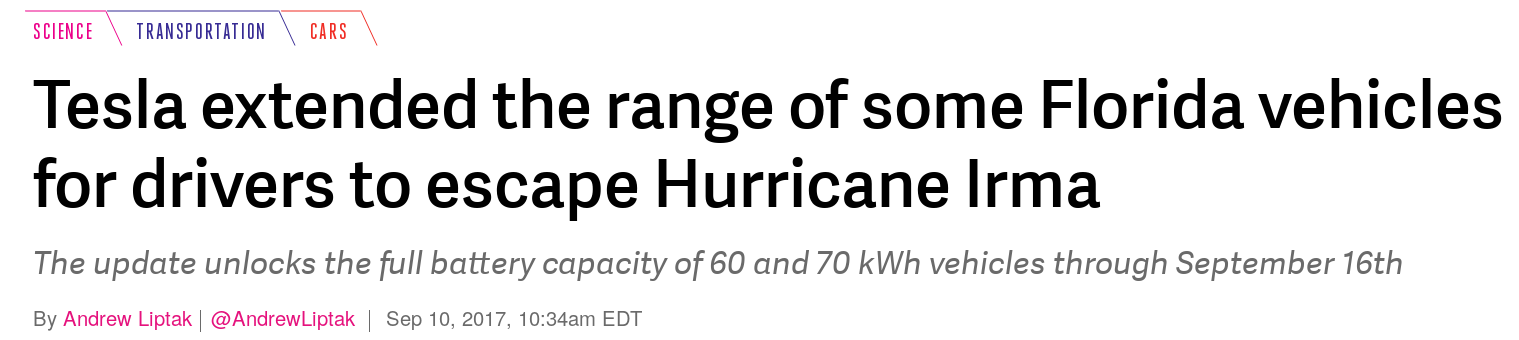
\includegraphics[width=12cm]{figs/tesla}
  \end{center}

  \begin{flushright}
    {\em
      \href{https://www.theverge.com/2017/9/10/16283330/tesla-hurricane-irma-update-florida-extend-range-model-s-x-60-60d}{The Verge} \\
      }
  \end{flushright}
  
\end{frame}

%% %%---------------------------------------------------------------

%% \begin{frame}
%% \frametitle{Teléfonos, libros, tabletas y otros cacharros}

%% Hemos considerado tan normal \\
%% no poder modificar el software de un teléfono...

%% \vspace{1cm}

%% \begin{flushright}
%% ...que las condiciones de iOS (iPhone) \\
%% parecieron aires de libertad
%% \end{flushright}

%% \end{frame}

%% %%---------------------------------------------------------------

%% \begin{frame}
%% \frametitle{Condiciones de instalación de software en i*}

%% \begin{itemize}
%% \item Sólo lo que Apple haya aprobado
%% \item Apps sólo del App Store
%% \end{itemize}

%% %\vspace{.5cm}

%%  (incluso si el teléfono es tuyo)

%% %\vspace{.5cm}

%%  (incluso si el programa es tuyo)

%% %\vspace{.5cm}

%%  (incluso si lo usas sólo tú)

%% %\vspace{.5cm}

%% \begin{flushright}
%%   ...aunque saltarse estas limitaciones técnicas \\
%%   podría ser legal
%% \end{flushright}
%% \end{frame}

%%---------------------------------------------------------------

\begin{frame}
\frametitle{Condiciones de instalación de software en i*}

%\begin{quote}
``Applications must not contain any obscene, pornographic, offensive or defamatory content or materials of any kind (text, graphics, images, photographs, etc.), or other content or materials that in Apple's reasonable judgment may be found objectionable by iPhone or iPod touch users''
%\end{quote}

\begin{flushright}
  {\footnotesize
    Section 3.3.14, iPhone Developer Program License Agreement
    }
\end{flushright}
\end{frame}

%%---------------------------------------------------------------

\begin{frame}
\frametitle{¿Quién decide qué puedes leer, qué puedes ver?}

\begin{itemize}
\item``5.000 aplicaciones relacionadas con el sexo eliminadas del App Store''  (febrero 2010)
  
\item Entre ellas, varios periódicos (marzo 2010)\\

\item Entre ellas, viñetas políticas ganadoras de Pulitzer (abril 2010)\\
\end{itemize}

  \begin{flushright}
    {\tiny
      \url{http://news.cnet.com/8301-13579_3-10457460-37.html}\\
      \url{http://gizmodo.com/5490310/its-time-to-declare-war-against-apples-censorship}\\
      \url{http://www.theregister.co.uk/2010/04/15/mark_fiore_rejected_from_app_store/}\\
    }
  \end{flushright}

\end{frame}


%%---------------------------------------------------------------

\begin{frame}
\frametitle{¿Quién decide qué puedes leer, qué puedes ver?}

  Tetas x tetas

\begin{center}
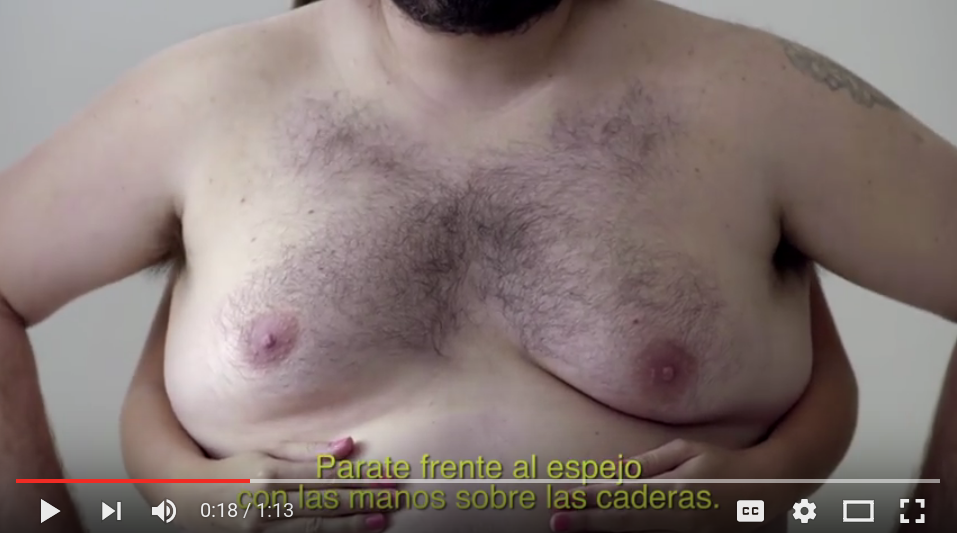
\includegraphics[height=4cm]{figs/tetasxtetas}
\end{center}

{\tiny \url{https://youtu.be/vOP9hEhYCek}}
\end{frame}


%% %%---------------------------------------------------------------

%% \begin{frame}
%% \frametitle{La nube decide qué puedes leer, y traza lo que haces}

%% \begin{itemize}
%% \item Páginas de Femen en Facebook cerradas por ``promover la prostitución''
%% \item Google SafeSearch filtra resultados de imágenes sin que siquiera te entereres
%% \item PRISM accede a datos almacenados de comunicaciones entre particulares
%% \end{itemize}
%% {\tiny
%%   \url{http://www.euronews.com/2013/06/26/facebook-said-femen-promotes-prostitution/}\\
%%   \url{http://www.zdnet.com/google-com-now-censors-explicit-content-from-image-searches-7000008705/}\\
%%   \url{http://en.wikipedia.org/wiki/PRISM_\%28surveillance_program\%29}\\
%% }
%% \end{frame}


%% %%---------------------------------------------------------------

%% \begin{frame}
%% \frametitle{Muchos otros casos...}

%% \begin{itemize}
%% \item Amazon borró libros comprados de los Kindle que los tenían
%% \item Facebook (y muchos otros) manejan nuestros datos personales
%% \item Facebook (y muchos otros) cierran cuentas ``por muchos motivos''
%% \item UEFI Secure Boot puede dificultar que instales Linux en tu ordenador
%% \item ...
%% \end{itemize}

%% \end{frame}

%%---------------------------------------------------------------

\begin{frame}
\frametitle{Cepillos de dientes chivatos}

\begin{center}
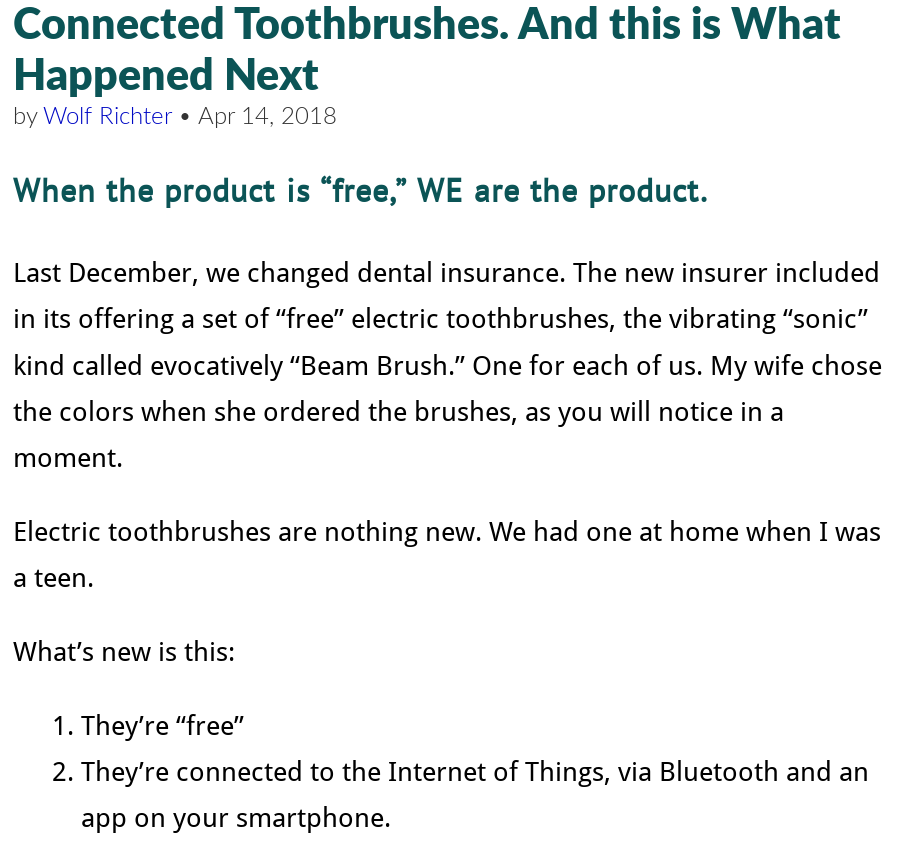
\includegraphics[height=5.8cm]{figs/toothbrushes}
\end{center}
\begin{flushright}
{\tiny \href{https://wolfstreet.com/2018/04/14/our-dental-insurance-sent-us-free-internet-connected-toothbrushes-and-this-is-what-happened-next/}{Our Dental Insurance Sent us “Free” Internet-Connected Toothbrushes}}
\end{flushright}

\end{frame}

%%---------------------------------------------------------------

\begin{frame}
\frametitle{Asistentes personales}

\begin{flushright}
  Google Now, Siri, Cortana (y muchos otros)
\end{flushright}

\begin{quote}
  ``Te aviso:
  ve saliendo para el aeropuerto \\
  porque tu avión despega en tres horas \\
  y hay un buen atasco en la M-40'' \\
\end{quote}

¿Cómo se puede conseguir esto?

\begin{flushright}
  {\tiny \href{http://searchengineland.com/how-google-now-siri-cortana-predict-what-you-want-229799}{How Google Now, Siri, Cortana predict what you want}}
\end{flushright}
\end{frame}

%%-----------------------------------------
\begin{frame}[fragile]

  \begin{center}
  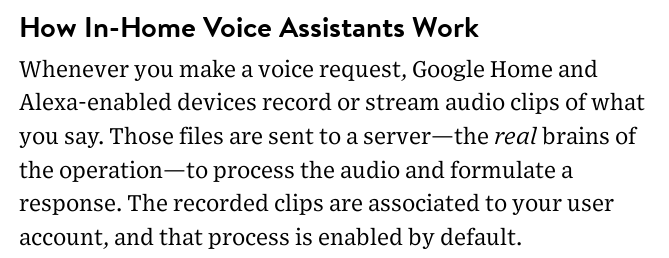
\includegraphics[width=10cm]{figs/home-assistants}
  \end{center}

  \begin{flushright}
    {\em
      \href{https://www.wired.com/2016/12/alexa-and-google-record-your-voice/}{Alexa and Google Home Record What You Say.} \\
      Wired \\
      }
  \end{flushright}
  
\end{frame}

%%-----------------------------------------
\begin{frame}[fragile]

  \begin{center}
  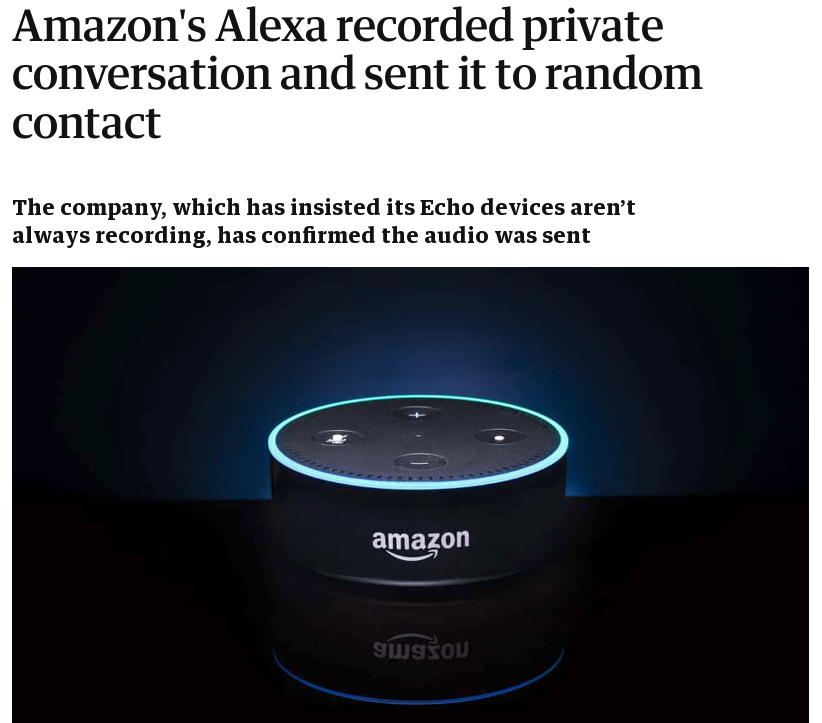
\includegraphics[width=8cm]{figs/alexa-recorded}
  \end{center}

  \begin{flushright}
    {\em \tiny
      \href{https://www.theguardian.com/technology/2018/may/24/amazon-alexa-recorded-conversation}{Amazon's Alexa recorded private conversation and sent it to random contact}}
  \end{flushright}
  
\end{frame}

%%-----------------------------------------
\begin{frame}[fragile]
\frametitle{Máquinas que curan... \\ y matan}

  \begin{center}
  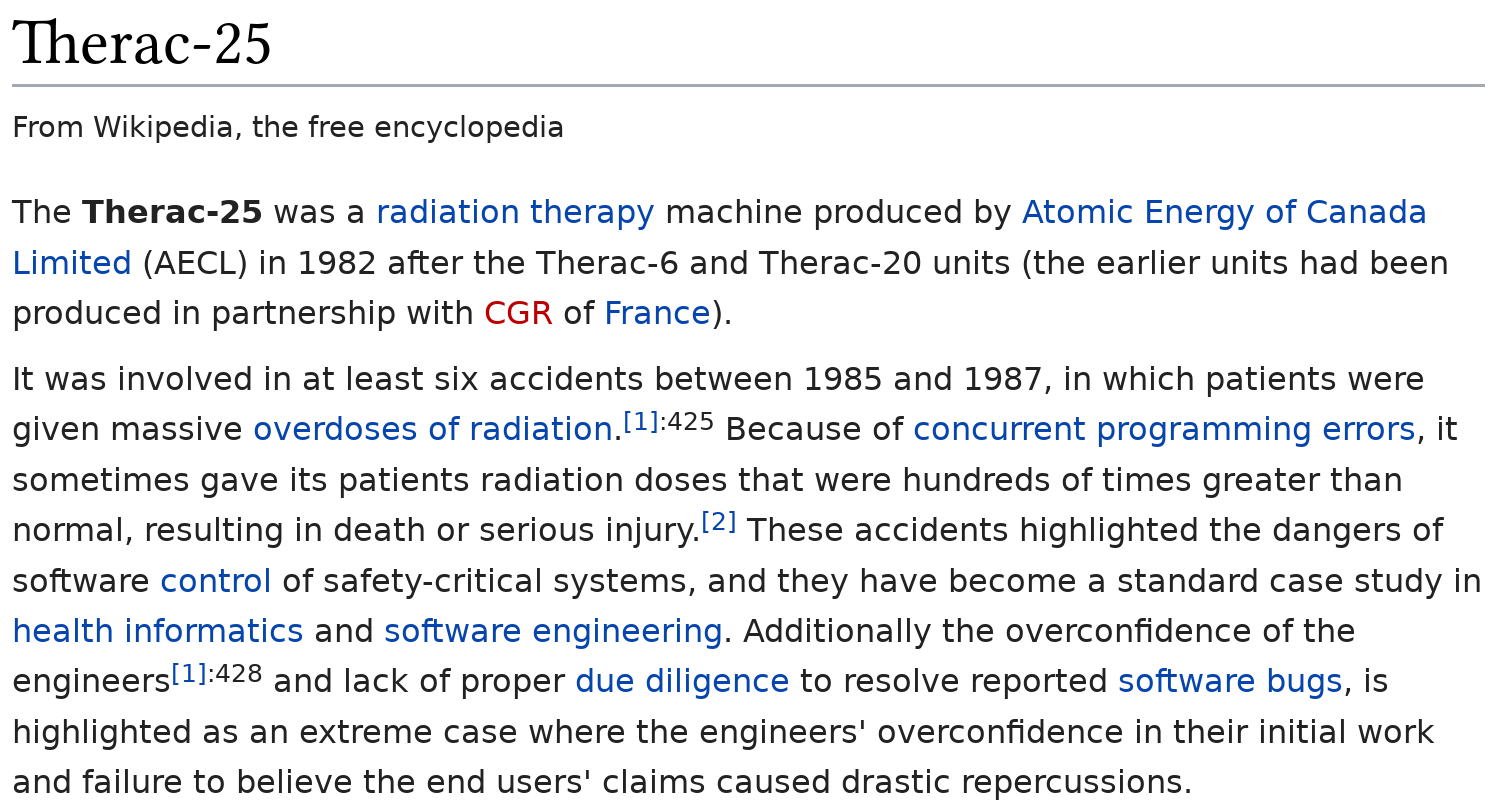
\includegraphics[width=8cm]{figs/therac-25}
  \end{center}

  \begin{flushright}
    {\em \tiny
      \href{https://en.wikipedia.org/wiki/Therac-25}{Therac-25 en Wikipedia}}
  \end{flushright}
  
\end{frame}

%%---------------------------------------------------------------

\begin{frame}
\frametitle{Y por supuesto...}

\begin{center}
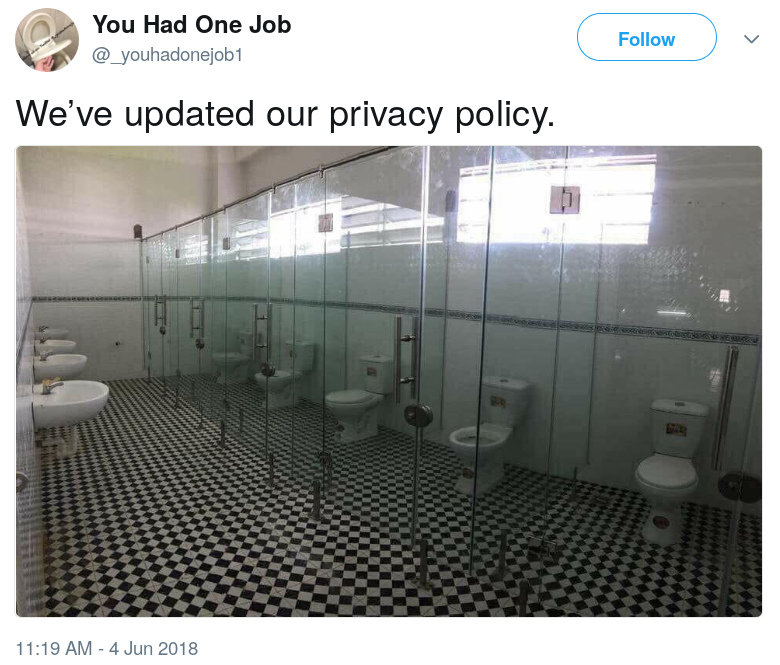
\includegraphics[height=7cm]{figs/privacy-policy-wc}
\end{center}

\end{frame}

%%---------------------------------------------------------------
%%---------------------------------------------------------------
\section{El problema}

%%---------------------------------------------------------------

\begin{frame}
\frametitle{¿Cuál es el problema?}

{\large
\begin{center}
No es que una empresa \\
haga estas cosas
\pause
\vspace{1cm}

Es que se puedan hacer
\pause
\vspace{1cm}

y que socialmente dejemos que se hagan
\end{center}
}
\end{frame}



%%---------------------------------------------------------------
%%---------------------------------------------------------------
\section{Tendencias}

%%---------------------------------------------------------------

\begin{frame}
\frametitle{Código y ley}

\begin{center}
  Históricamente, \\
  los sistemas legales han impuesto sus limitaciones. \\
  \vspace{1cm}
Ahora, los sistemas tecnológicos también. \\
  \vspace{1cm}
Muy frecuentemente se refuerzan entre ambos. \\
\end{center}

\end{frame}

%%-----------------------------------------
\begin{frame}[fragile]

  \begin{center}
  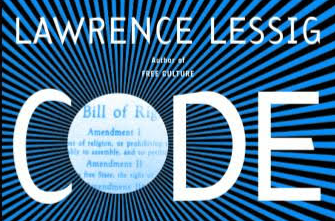
\includegraphics[width=10cm]{figs/code-is-law}
  \end{center}

  \begin{flushright}
``Codev2'', Lawrence Lessig \\
\url{http://www.codev2.cc/}
\end{flushright}

\end{frame}


%%---------------------------------------------------------------

\begin{frame}
\frametitle{La guerra sobre el ordenador generalista}

\begin{center}
El ordenador de propósito general podría convertirse en una anécdota en la historia \\
o no
\\
(se decidirá durante los próximos años) \\
\end{center}

\begin{flushright}
{\em \href{http://boingboing.net/2011/12/27/the-coming-war-on-general-purp.html}{The Coming War on General Purpose Computation}, \\
  Cory Doctorow} \\
\end{flushright}

\end{frame}


%%-----------------------------------------
\begin{frame}[fragile]

\begin{columns}
  \begin{column}{0.7\textwidth}
    {\em \small
    The line it is drawn \\
    The curse it is cast \\
    The slow one now \\
    Will later be fast \\
    As the present now \\
    Will later be past \\
    The order is rapidly fading \\
    And the first one now will later be last \\
    For the times they are a-changin' \\
    }
  \end{column}
  \begin{column}{0.3\textwidth}  %%<--- here
    \begin{center}
      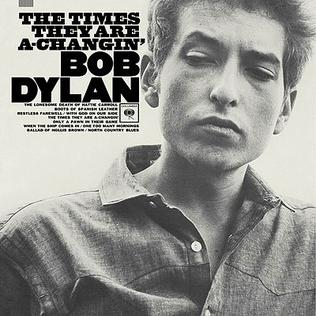
\includegraphics[width=\textwidth]{figs/The_Times_They_Are_a_Changin}
    \end{center}
  \end{column}
\end{columns}
  
\end{frame}


%%-----------------------------------------
\begin{frame}[fragile]
  \frametitle{Los tiempos están cambiando...}


  ¿Cuál será el próximo modelo de Internet?
  
\end{frame}

%%-----------------------------------------
\begin{frame}[fragile]
\frametitle{Un día cualquiera en unos años...}

  \begin{center}
  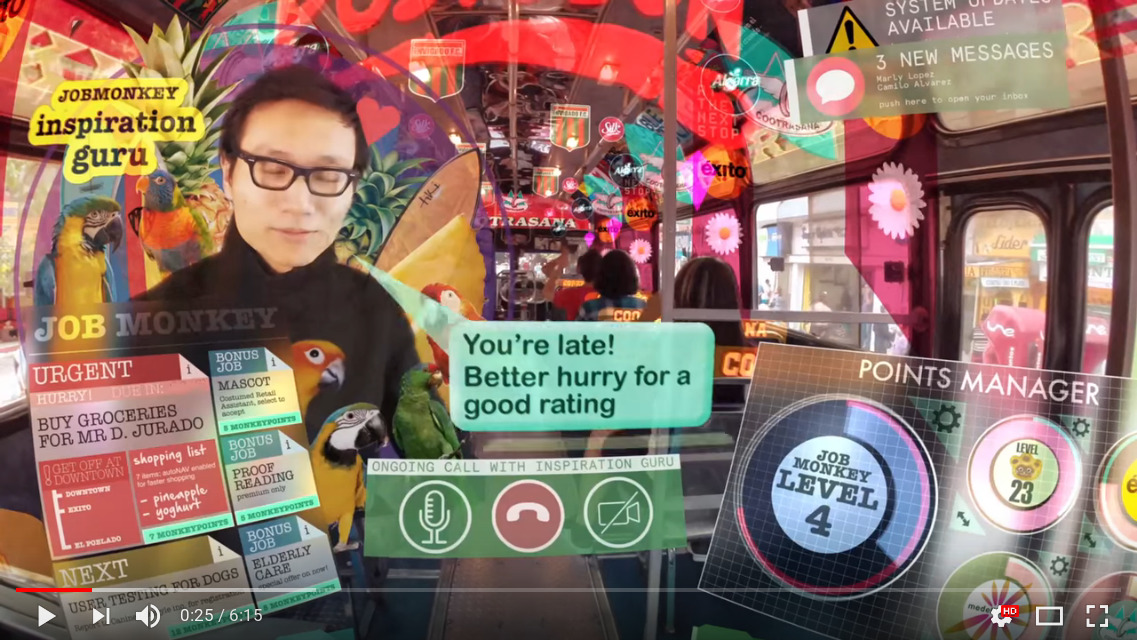
\includegraphics[width=8cm]{figs/hyper-reality}
  \end{center}

  \begin{flushright}
    {\em \tiny
      \href{https://www.youtube.com/watch?v=YJg02ivYzSs}{Hyper-reality}}
  \end{flushright}
  
\end{frame}

%%---------------------------------------------------------------

\begin{frame}
\frametitle{Una visión alternativa}

\begin{itemize}
\item Más cómputo y almacenamiento, \\
  más baratos, menos consumo, más movilidad \\
\item Más interconexión, más rápida, \\
  más barata \\
\item Mejores tecnologías federadas, \\
  extremo a extremo \\
\end{itemize}

  \begin{flushright}
  ¿Dispositivos personales \\
  interconectados directamente? \\
  \end{flushright}

\end{frame}

%%---------------------------------------------------------------

\begin{frame}
\frametitle{Tecnología y sociedad}

{\Large
La tecnología no es neutra: \\
Nos lleva hacia un cierto mundo \\
entre todos los posibles, \\
favoreciendo ciertos patrones \\
y dificultando otros \\
}

\end{frame}

%%---------------------------------------------------------------
%%---------------------------------------------------------------
% Wikimedia Commons
% Franklin D. Sergent who is 13 years old and in the fifth grade does his homework
% U.S. National Archives and Records Administration
% License: Public domain
% https://commons.wikimedia.org/wiki/File:Franklin_D._Sergent_who_is_13_years_old_and_in_the_fifth_grade_does_his_homework_-_NARA_-_541349.jpg
%% \renewcommand{\secimage}{figs/homework}
%% {\bf
%%   \textcolor[rgb]{1,1,1}{
%%     \section{Deberes para casa}
%%   }
%% }


%%---------------------------------------------------------------

\begin{frame}
\frametitle{Ejercicio: \\ aprende, controla, piensa...}


{\small
\begin{itemize}
  \item \url{http://www.google.com/settings/ads/}
  \item \url{https://maps.google.com/locationhistory}
  \item \url{https://www.google.com/history/}
  \item \url{https://www.google.com/settings/dashboard}
  \item \url{https://security.google.com/settings/security/permissions}
  \item \url{https://www.youtube.com/feed/history/search_history}
  \end{itemize}
}
\end{frame}

% Tip Jar, Alamo Beer
% Nan Palmer
% Wikimedia Commons
% https://commons.wikimedia.org/wiki/File:Tip_Jar,_Alamo_Beer_(2015-03-26_18.48.31_by_Nan_Palmer).jpg
% License: Creative Commons Attribution 2.0 Generic
\renewcommand{\secimage}{figs/tipjar}
{\bf
  \textcolor[rgb]{1,1,1}{
    \section{Propina}
  }
}

%%---------------------------------------------------------------

\begin{frame}
\frametitle{El ordenador, esa máquina maravillosa...}

Una herramienta posibilitadora:

\begin{itemize}
\item Permite realizar cualquier cosa que pueda hacer un programa
\item ...y los programas pueden hacer muchas cosas
\end{itemize}


\end{frame}

%%---------------------------------------------------------------

\begin{frame}
\frametitle{El ordenador, esa máquina maravillosa...}

Pero además...

\begin{itemize}
\item ...podemos instalar cualquier programa
\item ...podemos construir cualquier programa
\item ...podemos compartir cualquier programa
\item (o convencer a alguien para que lo construya)
\end{itemize}

\vspace{.2cm}

\begin{center}
Software y ordenador: conocimiento en acción
\end{center}
\end{frame}

%%---------------------------------------------------------------

\begin{frame}
\frametitle{...a la que imponemos limitaciones}

Pero se acepta que los programas vengan ``limitados'':

\vspace{.2cm}

\begin{itemize}
\item Limitaciones al uso
\item Limitaciones al entendimiento
\item Limitaciones a la distribución
\item Limitaciones a la modificación
\end{itemize}

\end{frame}

%%---------------------------------------------------------------

\begin{frame}

\begin{center}
\textbf{\Huge ¿Por qué aceptamos estas limitaciones?}
\end{center}
\end{frame}

%%---------------------------------------------------------------

\begin{frame}
\frametitle{Algunos visionarios cambiaron el mundo}

A principios de los 1980s hubo quien se hizo esta pregunta...

\vspace{.1cm}

...y se propuso mostrar cómo el software libre nos empodera.

\vspace{.1cm}

Las implicaciones son enormes

\begin{flushright}
{\small \url{http://www.gnu.org/philosophy/free-sw.html}}
\end{flushright}
\end{frame}

%%---------------------------------------------------------------

\begin{frame}
\frametitle{El software libre puedes...}

{\large
\begin{itemize}
\item usarlo como mejor te parezca
\item redistribuirlo a quien quieras
\item modificarlo (mejorarlo, adaptarlo)
\item redistribuir las modificaciones
\end{itemize}
}
\end{frame}

%%---------------------------------------------------------------

\begin{frame}
\frametitle{Consecuencias}

\begin{itemize}
\item Cualquiera tiene acceso al conocimiento \\
  ...cualquiera puede adaptar, modificar, innovar incrementalmente
\item Cualquiera tiene acceso a la herramienta \\
  ...cualquiera puede utilizarla para sus fines
\item Cualquiera puede colaborar \\
  ...liberación de potenciales en comunidades de innovación
\end{itemize}

\end{frame}

%%---------------------------------------------------------------

\begin{frame}
\frametitle{Y la realidad cambió...}

{\Large
\begin{center}
  Hoy día, \\
  el software libre es una realidad: \\
  la infraestructura \\
  verdaderamente común de la \\
  sociedad de la información \\
\end{center}
}
\end{frame}

%%---------------------------------------------------------------
% LICENCIA DE REDISTRIBUCION DE LAS TRANSPAS
\frame{
~
\vspace{3cm}

\begin{flushright}
{\small
\copyright 2012-2018 Jesús M. González Barahona. \\

  Algunos derechos reservados. \\
  Este artículo se distribuye bajo la licencia \\
  ``Reconocimiento-CompartirIgual 3.0 España'' \\
  de Creative Commons, \\
  disponible en \\
}
{\footnotesize
  \url{https://creativecommons.org/licenses/by-sa/3.0/es/} \\
}
\end{flushright}
}

\end{document}
